\section{Experimentos}
Comparamos nossas implementações com o
\gzip\footnote{\url{http://www.gzip.org/}},
grep\footnote{\url{https://www.gnu.org/software/grep/}} e com o
codesearch\footnote{\url{https://github.com/google/codesearch}}.
Realizamos experimentos para responder às seguintes perguntas:
\begin{enumerate}
\item \rqone
\item \rqtwo
\item \rqthree
\end{enumerate}

Foram implementados scripts em BASH para controlar os experimentos e fazer
medições, gerando arquivos .raw de saída contendo resultados. Foram também
implementados scripts em R que desenham gráficos de acordo com os arquivos .raw
gerados pelos scripts BASH.


Todos os experimentos foram realizados em uma máquina com processador Intel Core
i5 2.6Ghz e 8Gb de RAM. Cada medição de tempo nos experimentos foi realizada 10
vezes, e somente a média foi considerada e reportada nos resultados.
Todos os scripts e resultados estão disponíveis no diretório {\it experiments}.

\subsection{\rqone}
Nós comparamos a nossa implementação do \lz com o \gzip em dois aspectos: Tempo
e taxa de compressão.
Para realizar essa comparação, nós dividimos um arquivo\footnote{
\url{http://pizzachili.dcc.uchile.cl/texts/nlang/english.1024MB.gz}}
que contém 1GB de texto em inglês em arquivos de
tamanhos distintos: 100KB, 200KB, 300KB, 700KB, 1MB, 2MB, 3MB, 5MB, 50MB, 100MB,
200MB, 300MB e 500MB. Cada arquivo desse contém os primeiros n bytes do
arquivo original, onde n é o tamanho do arquivo.

\subsubsection{Tempo}

Abaixo está um gráfico que relaciona o tempo que leva para comprimir um arquivo
com o tamanho dele, para ambos o nosso \lz e o \gzip.
\\
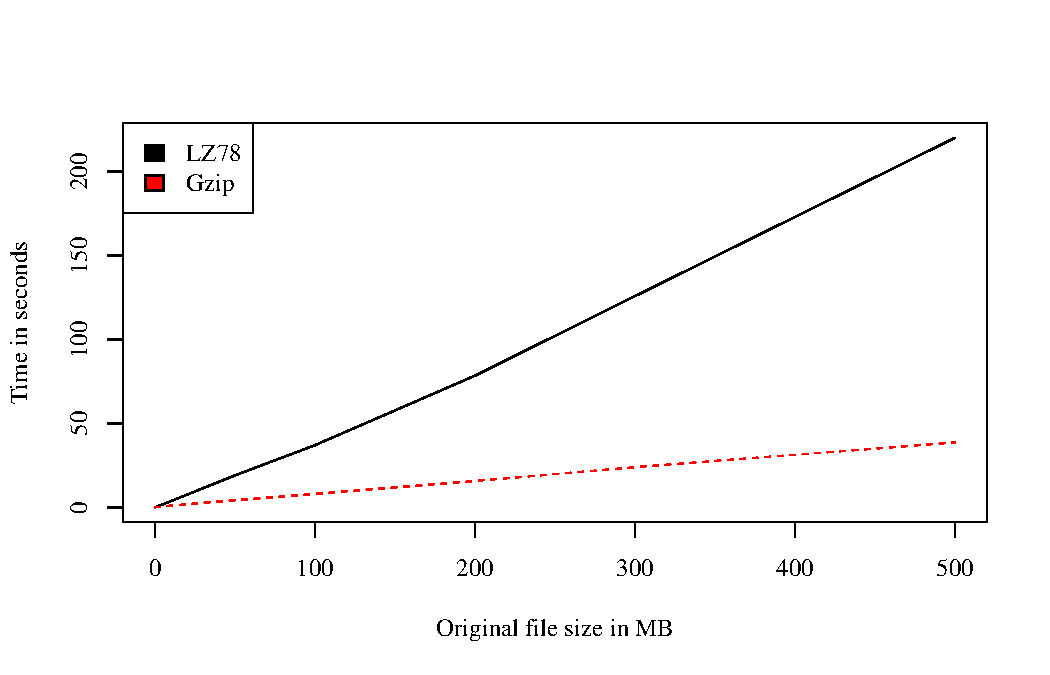
\includegraphics[scale=0.74]{../experiments/R/pdf/time_comp}
\\

Ambas as funções são (ou se aproximam muito de) retas, o que comprova que a
nossa implementação do \lz, bem como o \gzip, comprimem em tempo linear de
acordo com o tamanho do arquivo. Porém, a constante que multiplica a função do
\gzip é bem menor do que a nossa. Isso acontece porque o \gzip está em
desenvolvimento a mais de 23 anos, onde experts estão sempre otimizando o
algoritmo, fazendo com que essa constante da função linear seja cada vez menor.


Os arquivos comprimidos acima foram descomprimidos com ambas as ferramentas \lz
e \gzip. Abaixo está um gráfico que relaciona o tempo que leva para descomprimir
um arquivo e o tamanho dele.
\\
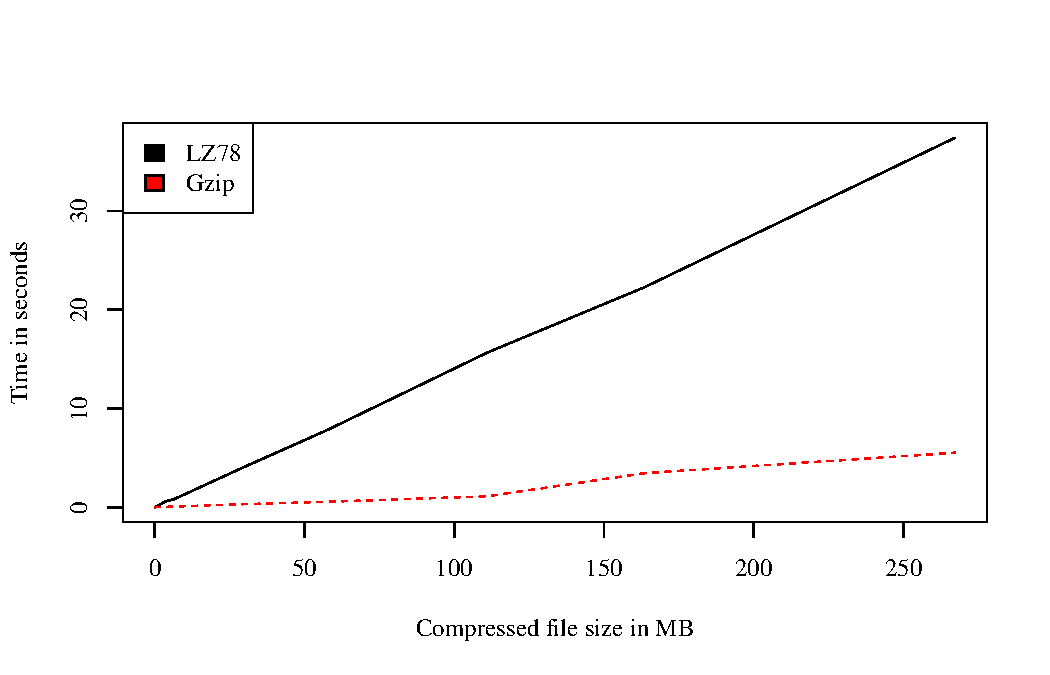
\includegraphics[scale=0.74]{../experiments/R/pdf/time_decomp}
\\

Obtivemos novamente um resultado consistente com o anterior: ambos possuem
complexidade linear, porém a constante da descompressão do \gzip é muito
superior à da nossa implementação. Isso ficou ainda mais acentuado na
descompressão do que na compressão.

\subsubsection{Taxa de compressão}

Abaixo está um gráfico que relaciona a taxa de compressão de um arquivo com o
tamanho original dele, para ambos o nosso \lz e o \gzip.
\\
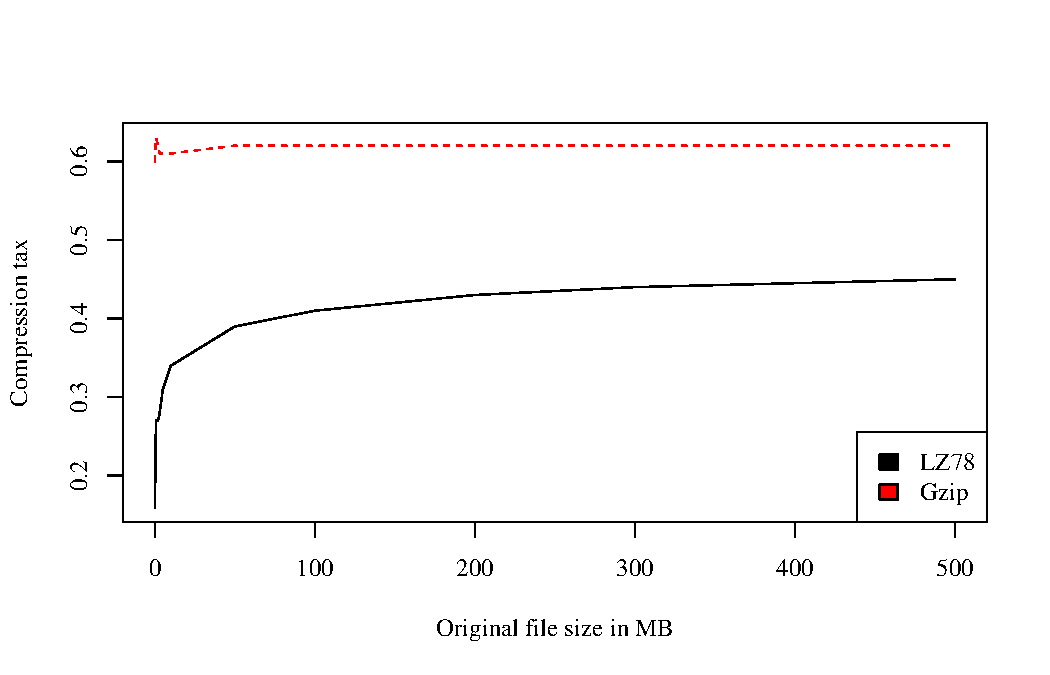
\includegraphics[scale=0.74]{../experiments/R/pdf/comp_tax}
\\

Novamente, os resultados se assemelham quando analisados separadamente:
Ambos possuem uma variação inicial (apesar do \gzip ter uma bem menor) e se
estabilizam para arquivos maiores. Porém, o \gzip se estabiliza com uma taxa de
compressão próxima de 60\%, enquanto que o nosso \lz se estabiliza com uma taxa
próxima de 42\%. Recorremos novamente ao argumento de que o \gzip está em
desenvolvimento a muito mais tempo e por isso possui mais otimizações.

\subsection{\rqtwo}
Para responder à essa pergunta nós utilizamos a ferramenta \ipmt para criar um
índice de um arquivo de texto. Após isso comparamos o tempo de realizar buscas
de diversos padrões utilizando \ipmt no arquivo indexado e comparando com o
tempo para pesquisar os padrões utilizando grep no texto original.

Nós consideramos somente o arquivo de 50MB pelo seguinte motivo: O arquivo .idx
gerado pela ferramenta \ipmt possui ambos o texto original e o índice
comprimidos. Acontece que o array do nosso LSA tem, em média, quase 10 vezes o
tamanho do arquivo original. Ou seja, indexar e comprimir um arquivo de 50MB
acaba se tornando uma tarefa de comprimir um arquivo de aproximadamente 500MB,
que dura pouco mais de 4 minutos. Nesse caso, nossa compressão criou um arquivo
.idx de 341MB, onde as buscas serão realizadas. Indexar e comprimir arquivos
maiores do que 50MB é uma tarefa custosa para nossas implementações.



\subsection{\rqthree}

\todo{add text}

